%!TEX root = lab6.tex

\setcounter{chapter}{6}
\chapter*{Introduction}

Before diving into this computer networks lab course, it is useful to present some conventions first. \stress{Keep in mind that these conventions are introduced to make all of our lives easier.} In case of problems, it is easier to have a look at a lab setup if everyone sticks to the same rules.

\section{Practical Arrangements}

\subsection{Virtual Machine with NS-3}

\subsubsection{Getting the VM}
We provide a Virtual Machine with an Ubuntu variant and NS-3 installed. You can download this image from \url{https://student.idlab.uantwerpen.be/computernetwerken/}. There are two distinct VMs available: one for running on Intel-based computers (``Computernetwerken-AMD64''), and one for running on Apple silicon (``Computernetwerken-ARM'').

If you are using a computer running on Intel architecture, we suggest you use Virtualbox (\url{https://www.virtualbox.org/}) for running your Virtual Machine. After installing Virtualbox, set up your machine as follows:
\begin{enumerate}
\item Download and open the Computernetwerken-AMD64.ova file.
\item You should now see the VirtualBox Import Appliance.
\item Click the Import button, and the Virtual Machine is imported in Virtualbox. This can take a few minutes.
\end{enumerate}

When you are using a machine running on Apple silicon, A VM is provided that has been made with the ``UTM'' virtualisation software. UTM is freely downloadable from \url{https://getutm.app}. If your are using Apple silicon, set up your machine as follows after installing the UTM appliance:
\begin{enumerate}
	\item Download and open the Computernetwerken-ARM.utm.zip file.
	\item Unpack the zip file.
	\item You should now see the UTM Appliance.
	\item Double-click the Computernetwerken-ARM.utm file to import it into UTM.
	\end{enumerate}

Now you should be able to start your virtual machine. The login is \incommand{computernetwerken}, and the password is \incommand{mvkbj1n} (from the Dutch phrase \emph{``Met veel kabels bouw je 1 netwerk''}).

\newpage
\section{NS-3: Introduction}\label{sec:lab0}
In this lab, you will acquaint yourself with the NS-3 simulation platform. Using this model, you will simulate two medium access control (MAC) layer protocols, Aloha and DCF, which specify how multiple devices of the same wireless network can access the medium. The modification of the latter one is used in modern wireless local area networks that we all know under the name Wi-Fi. 

\subsection{Basics of NS-3}
NS-3 is a discrete-event network simulator, targeted primarily for research and education use. This is a free open source software written in the C++ programming language. Using NS-3, you can conduct experimental studies on different communication technologies and network topologies. It contains implementations of protocols that are parts of many commonly used telecommunication technologies, for example, Wi-Fi and LTE/5G. The NS-3 repository can be accessed at \url{https://gitlab.com/nsnam/ns-3-dev/}, all the information and documentation can be found at \url{https://www.nsnam.org/}.

It is important to understand the difference between emulation and simulation: Mininet is a network emulator, while NS-3 is a simulator. Emulators work in real time and precisely mimic the behavior of real hardware and software in a real environment. In contrast, simulators maintain their own simulation clock and do not precisely follow all the procedures that occur in real devices and software. However, they approximate the environment and the devices behavior in an efficient way so that they provide a good accuracy of the experiment outcomes. For example, NS-3 does not emulate all operation system (e.g., Linux) procedures. It also does not emulate the signal generation and transmission over the wireless channel, but uses mathematical equations to estimate the error probability. Another very important feature provided by simulators is the experiment repeatability. It means that two or more runs of the simulation model with the same parameters will produce precisely the same results. Any randomness in a simulation model occurs due to the use of pseudorandom numbers to generate a certain event (see implementation details at \url{https://www.nsnam.org/docs/manual/html/random-variables.html}), e.g., error during data transmission event with a known probability obtained from an equation.

\begin{exercise}{Building and running NS-3}
This exercise walks you through the steps of building NS-3 and running an experiment (see also NS-3 tutorial \url{https://www.nsnam.org/docs/tutorial/html/}). The exercise is conducted on the virtual machine.

\begin{enumerate}
	\item NS-3 uses the Cmake system to build the project. To make the configuration and building easier for users, it provides a Python wrapper around Cmake, called ns-3, that symplifies the command-line syntax. You can find this wrapper in the root directory of the project, in our case it is \nolinkurl{~/ns3-student}. There are several options to control the build, e.g., enabling tests and examples, debug mode, etc. We will use the default build configuration. This is done by executing the following command:
	\begin{cmdblock}[gobble=2]
		% ./ns3 configure
	\end{cmdblock}
	When the command finishes execution, you should see the output in command line similar to the one on Fig.~\ref{fig:lab7-ns3-configure}.
	\begin{figure}[ht]
		\centering
		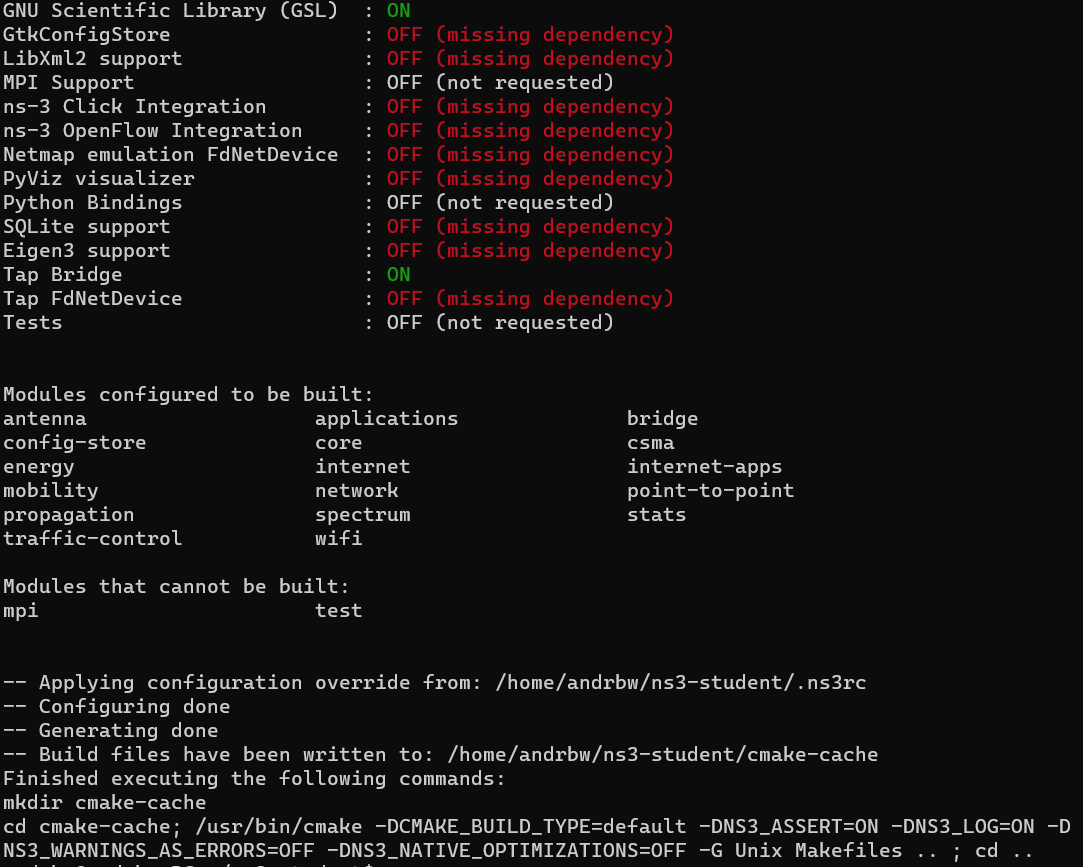
\includegraphics[width=0.8\linewidth]{graphics/ns3-configure}	
		\caption{NS-3 build configuration.}
		\label{fig:lab7-ns3-configure}
	\end{figure}

	\item Now we can build the NS-3 project. In directory \nolinkurl{~/ns3-student/src} we can see many subdirectories, each of which contains source files for a particular module of NS-3. Since not all of the modules will be required for our experiments, we will not build all of them. The configuration file \nolinkurl{~/ns3-student/.ns3rc} is used to configure the list of modules that we want to build. In our case, we build the following modules: 
	
	\begin{itemize}
		\item applications (for simple UDP application that we will use to generate data);
		\item bridge (contains implementation of switch);
		\item config-store (to configure parameters of different modules);
		\item core (the core of the simulator itself);
		\item csma (for ethernet);
		\item internet (\ac{ip}, \ac{udp}, \ac{arp} and other protocols of the internet stack);
		\item internet-apps (for ping);
		\item mobility (for setting positions of the devices);
		\item network (all main simulator abstractions are implemented in this module, i.e., packet, network device, header, etc.);
		\item propagation (for modeling of the physical channel);
		\item wifi (for implementation of wifi).
	\end{itemize}
	
	Build the project with the following command:
	\begin{cmdblock}[gobble=2]
		% ./ns3 build
	\end{cmdblock}
	Note that NS-3 will build using multiple threads, thus all or most of your CPUs will become busy. If you want to limit the number of parallel threads, e.g., to 10, use parameter -j:
	\begin{cmdblock}[gobble=2]
		% ./ns3 build -j 10
	\end{cmdblock}
	When the command finishes execution, you should see output on command line similar to the one on Fig.~\ref{fig:lab7-ns3-build}.
	\begin{figure}[ht]
		\centering
		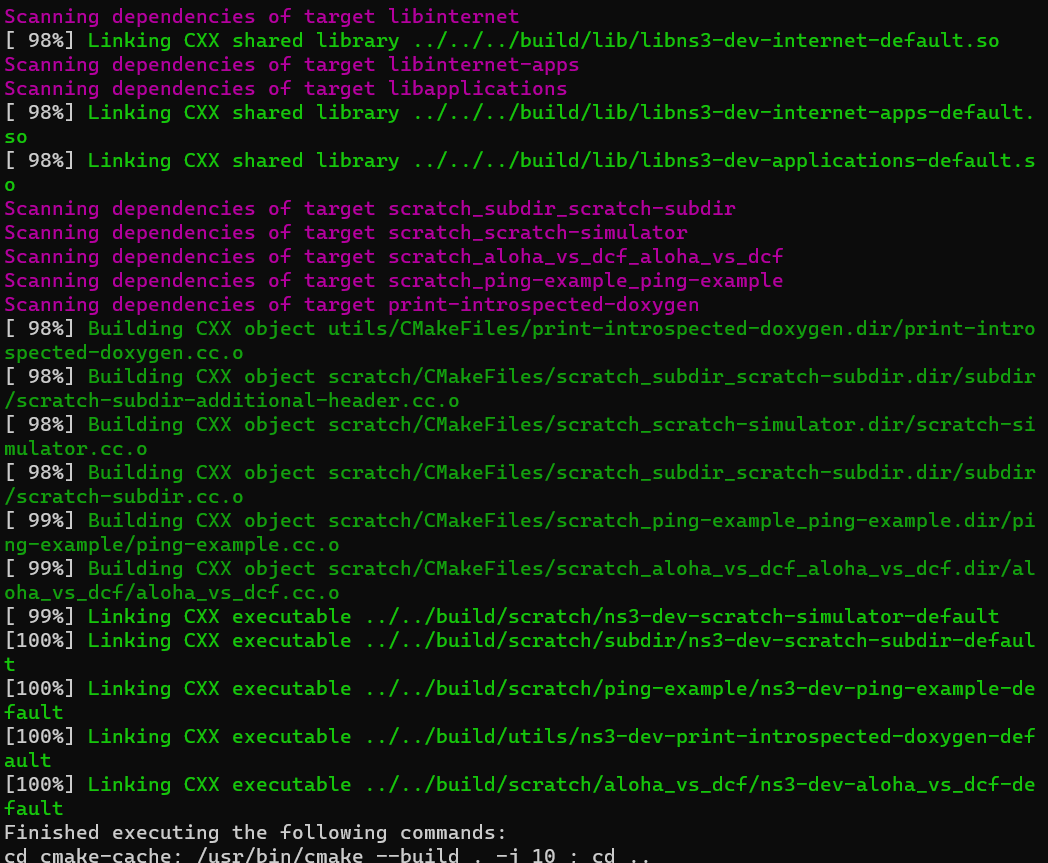
\includegraphics[width=0.8\linewidth]{graphics/ns3-build}	
		\caption{NS-3 build execution.}
		\label{fig:lab7-ns3-build}
	\end{figure}
		
	\item To test if the build process was successful, we will run a test experiment. Go to directory \nolinkurl{~/ns3-student/scratch/ping-example} and execute the following command (the PWD command returns the full pathname of the current working directory):
	\begin{cmdblock}[gobble=2]
		% ./../../ns3 run --cwd=$PWD "ping-example"
	\end{cmdblock}
	Here we use the parameter cwd to specify the working directory, which NS-3 will use for all relative paths, e.g., to read from files or print to them. By default, the working directory is the root directory of the NS-3 project. If the experiment is finished correctly, you will see the same output as in Fig.~\ref{fig:lab7-ping-testrun}. Besides, multiple pcap traces will appear in the directory.
	\begin{figure}[ht]
		\centering
		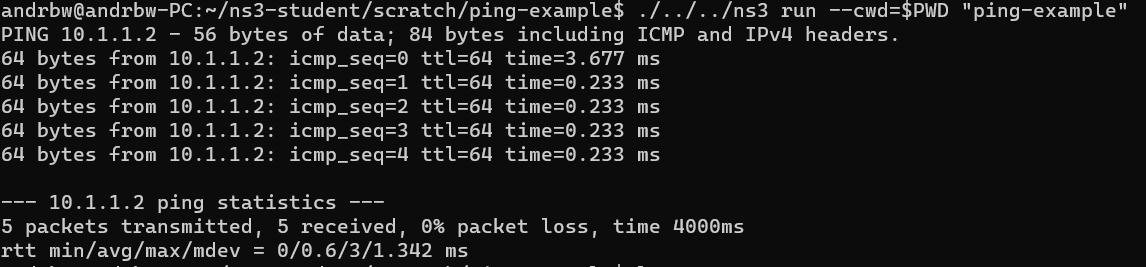
\includegraphics[width=0.8\linewidth]{graphics/ping-testrun}	
		\caption{Output generated by ping-example experiment run.}
		\label{fig:lab7-ping-testrun}
	\end{figure}
\end{enumerate}

\end{exercise}

\begin{exercise}{Building a simple \textbf{wired} topology and executing the ping command}
	In this exercise, we will go deeper into the ping-example experiment. Specifically, we will learn how to create a simple wired topology in NS-3 and execute a ping command to initiate an exchange of \ac{icmp} packets between the nodes. The network setup in Fig.~\ref{fig:lab7-ping-wired} and Tab.~\ref{tab:lab7-ping-addr} is used in this exercise.
	\begin{figure}[ht]
		\centering
		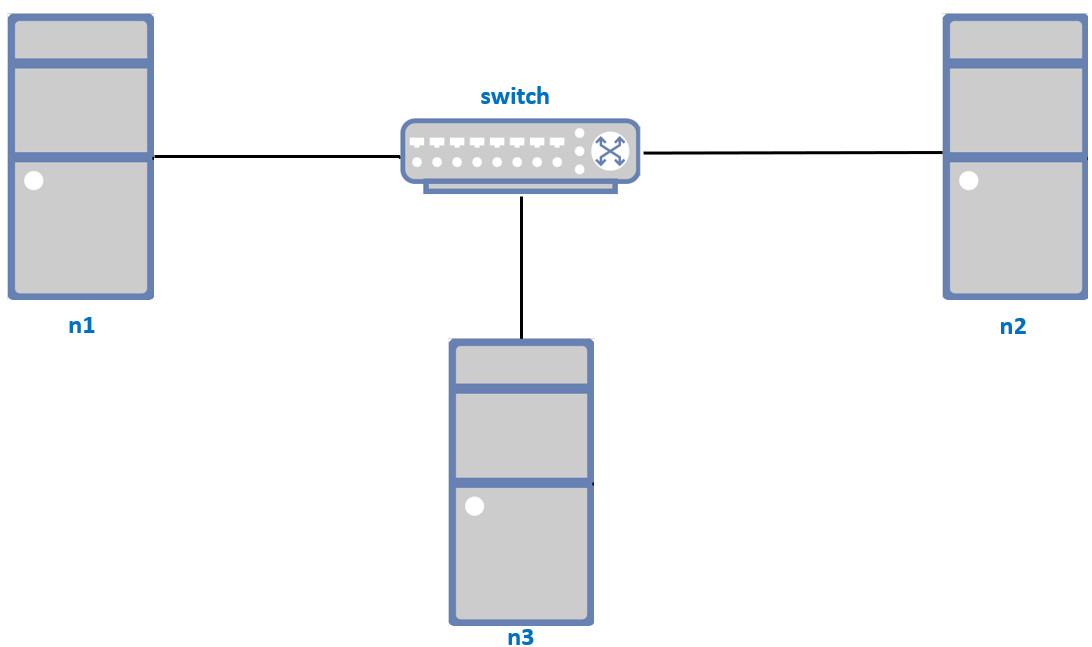
\includegraphics[width=0.5\linewidth]{graphics/ping-wired-topology}	
		\caption{Wired network topology in ping-example experiment.}
		\label{fig:lab7-ping-wired}
	\end{figure}
	\begin{table}[ht]
		\centering
		\begin{tabular}{| c | c | c |}	
			\hline
			\textbf{End node} & \textbf{\ac{ip} address} \\ \hline
			n1 & \ipaddr{10.1.1.1/24} \\ 
			n2 & \ipaddr{10.1.1.2/24} \\ 
			n3 & \ipaddr{10.1.1.3/24} \\ \hline
		\end{tabular}
		\caption{\acs{ip} addresses of the hosts.}
		\label{tab:lab7-ping-addr}
	\end{table}

	\begin{enumerate}
		\item When we run an experiment in NS-3, we can set its parameters via the command line. For that, the class CommandLine is used. In experiment ping-example.cc, we have the following structure of the command line arguments:
		\begin{lstlisting}
		CommandLine cmd;
		cmd.AddValue("interval", "The time to wait between two packets", interPacketInterval);
		cmd.AddValue("size", "Data bytes to be sent, per-packet", size);
		cmd.AddValue("count", "Number of packets to be sent", count);
		cmd.AddValue("srcIdx",
		"End node index that is ping source, e.g., if 1 the src IP is \"10.1.1.1\"",
		srcIdx);
		cmd.AddValue("dstIdx",
		"End node index that is ping source, e.g., if 1 the src IP is \"10.1.1.2\"",
		dstIdx);
		cmd.Parse(argc, argv);
		\end{lstlisting} 
		Each function call AddValue has three arguments: the parameter name, its text description and reference to a variable to be set. For any experiment, we can always see the description of its variables by executing the run command with argument PrintHelp:
		\begin{cmdblock}[gobble=2]
			% ./../../ns3 run --cwd=$PWD "ping-example --PrintHelp"
		\end{cmdblock}
	
		If we do not specify any arguments after ping-example, the variables will not be changed. That means that their default values will be used. If we want to change the value of a particular variable, we can always specify its value in the run command:
		\begin{cmdblock}[gobble=2]
			% ./../../ns3 run --cwd=$PWD "ping-example --count=10"
		\end{cmdblock}
		
		\question{Using the description of the command line arguments and the output of the experiment run, describe what the experiment does by default.}{0}
		
		\item To create the devices and connect them with links, we use multiple NS-3 abstractions. The basic computing device abstraction is called Node. When you want to connect a real non-simulated computer to a network, you have to use a Network Interface Card (NIC). To control this hardware, network device software drivers are used. In NS-3, the NetDevice abstraction is used to cover both the software driver and the simulated NIC hardware. A NetDevice is “installed” in a Node in order to enable the Node to communicate with other Nodes in the simulation via Channels. Just as in a real computer, a Node may be connected to more than one Channel via multiple NetDevices. Just as an Ethernet NIC is designed to work with an Ethernet network, the CsmaNetDevice is designed to work with a CsmaChannel and a WifiNetDevice is designed to work with a WifiChannel.
		
		In our experiment, we will use CsmaHelper to create links between pairs of devices. Each link that we create has 100 Mbps data rate and 50\textmu s delay. Since we have three links, in total we will create 6 NetDevices: 1 installed on each of the end nodes and 3 installed on the switch device. To enable switch capabilities on a switch node, we also use BridgeHelper. The following code is responsible for the described procedure:
		\begin{lstlisting}
		NodeContainer endNodes;
		endNodes.Create(3);
		
		NodeContainer switchNode;
		switchNode.Create(1);
		
		CsmaHelper ethernet;
		ethernet.SetChannelAttribute("DataRate", StringValue("100Mbps"));
		ethernet.SetChannelAttribute("Delay", StringValue("50us"));
		
		NetDeviceContainer endNodeDevices;
		NetDeviceContainer switchDevices;
		for (int i = 0; i < 3; i++)
		{
		NetDeviceContainer linkDevices = ethernet.Install(NodeContainer (endNodes.Get (i), switchNode));
		endNodeDevices.Add (linkDevices.Get (0));
		switchDevices.Add (linkDevices.Get (1));
		}
		
		BridgeHelper bridge;
		bridge.Install(switchNode.Get (0), switchDevices);
		\end{lstlisting}
		
		\question{If we transmit a 100 bytes packet from node n1 to n2, and node n2 immediately transmits the same packet back to n1, what will be the round-trip time?}{0} 
				
		\item In this experiment, the exact positions of the nodes are not important. For simplicity, we place all of them to the same point: (0, 0, 0). For that, we use ListPositionAllocator with only one position in its list. Then, on each installation it will set this position to each node. Since we do not want the nodes to move, we use ConstantPositionMobilityModel. The following code is responsible for the described procedure:
		\begin{lstlisting}
		MobilityHelper mobility;
		Ptr<ListPositionAllocator> positionAlloc = CreateObject<ListPositionAllocator> ();
		positionAlloc->Add (Vector (0.0, 0.0, 0.0));
		mobility.SetPositionAllocator (positionAlloc);
		mobility.SetMobilityModel ("ns3::ConstantPositionMobilityModel");
		mobility.Install (endNodes);
		mobility.Install (switchNode);
		\end{lstlisting}
		
		\item To enable support of all main internet protocols, we use InternetStackHelper. Then, we use Ipv4AddressHelper to assign \ac{ipv4} addresses to all nodes.
		\begin{lstlisting}
		InternetStackHelper internet;
		internet.Install(endNodes);
		
		Ipv4AddressHelper ipv4;
		ipv4.SetBase("10.1.1.0", "255.255.255.0");
		ipv4.Assign(endNodeDevices);
		Ipv4InterfaceContainer interfaces = ipv4.Assign(endNodeDevices);
		\end{lstlisting}
		
		\item Finally, we install the ping tool on one of the nodes (with index srcIdx) where we want to execute the ping command. We set the following parameters: destination IP address, the size of the ICMP packets, the interval between packets, the number of packets to be sent (using the parameter ``Count''), the start time and the end time of the ping command execution. We also enable pcap files collection so that we can analyse the traffic captured on all devices during the experiment.
		\begin{lstlisting}
		PingHelper pingHelper(interfaces.GetAddress (dstIdx), interfaces.GetAddress (srcIdx));
		pingHelper.SetAttribute("Interval", TimeValue(interPacketInterval));
		pingHelper.SetAttribute("Size", UintegerValue(size));
		pingHelper.SetAttribute("Count", UintegerValue(count));
		ApplicationContainer apps = pingHelper.Install(endNodes.Get(srcIdx));
		apps.Start(Seconds(1));
		apps.Stop(Seconds(50));
		
		ethernet.EnablePcapAll("ping-example");
		\end{lstlisting}
		\remark Note that we do not install the ping tool on the receiver side. The tool is responsible for sending the ICMP echo requests, and output generation after interpreting the echo replies. However, generation of echo reply on a received echo request is a responsibility of ICMP protocol itself, so this procedure does not require the ping tool installation.
		
		\question{How many pcap files will be generated by the experiment? Why?}{0}
		
		\item The last part is often the same in all experiments. It consists of three commands: Stop, Run and Destroy. The Stop command creates the terminating event at a specific time moment that corresponds to the end of simulation. The Run command starts simulation, i.e., starts processing of the first event in the events queue. Finally, the Destroy command destroys all the objects that have been created during the experiment.
		\begin{lstlisting}
		Simulator::Stop(Seconds(60.0));
		Simulator::Run();
		Simulator::Destroy();
		\end{lstlisting}
		
		\item Now, when you understand the structure of the experiment, run the experiment with the following parameter configuration: send 8 ICMP ping packets from node with IP address 10.1.1.3 to node with IP address 10.1.1.1, set interval between packets to 0.5 seconds and packet size to 56 bytes. \textbf{Do not modify any source file!} Save the program output and the generated pcap files.
		
		\question{Which command did you use to run the experiment?}{0}
		
		\question{Look inside the content of each pcap file. Which packets do you see inside them? Do all the pcap files contain the same packets? Why?}{0}
		
		\item Modify the source file of the experiment, \nolinkurl{ping-example.cc}: add function call \\ ArpCache::PopulateArpCache () right after the \ac{ipv4} addresses assignment.
		\begin{lstlisting}
		Ipv4AddressHelper ipv4;
		ipv4.SetBase("10.1.1.0", "255.255.255.0");
		ipv4.Assign(endNodeDevices);
		Ipv4InterfaceContainer interfaces = ipv4.Assign(endNodeDevices);
		
		<@\textcolor{red}{ArpCache::PopulateArpCache ();}@>
		
		//Create Ping application and installing on node 
		\end{lstlisting}
		Run the experiment from the previous task again with the same parameters. Note that before running the experiment NS-3 will rebuild the file, because we changed it. Save the program output and the generated pcap files.
		
		\question{Is there any difference in program output and pcap files compared to the previous task? What does the function ArpCache::PopulateArpCache () do to cause such difference?}{0}
	\end{enumerate}
\end{exercise}

\begin{exercise}{Building simple \textbf{wireless} topology and executing the ping command}
	In this exercise, we will modify the experiment file \nolinkurl{ping-example.cc}. Specifically, we will substitute the wired topology with the wireless one. We will consider an older Wi-Fi wireless technology, that is standardized as IEEE 802.11a. The newest Wi-Fi standard is IEEE 802.11ax, that is commonly known as Wi-Fi 6. However, for simplicity we will configure an older version, it will be enough for our investigation purposes. 
	
	Since we will make all devices capable of communicating via wireless medium, we will no longer need the switch. Wi-Fi networks can operate in two modes: infrastructure and ad-hoc. Infrastructure mode is a very common mode that we are using at our homes when we connect all Wi-Fi devices to an access point. However, the presence of the access point is not necessary, because the devices can communicate with each other directly. For the sake of simplicity, we will consider this second mode, called \textbf{ad-hoc}. Then the network topology becomes very simple (see Fig.~\ref{fig:lab7-ping-wireless}).
	\begin{figure}[ht]
		\centering
		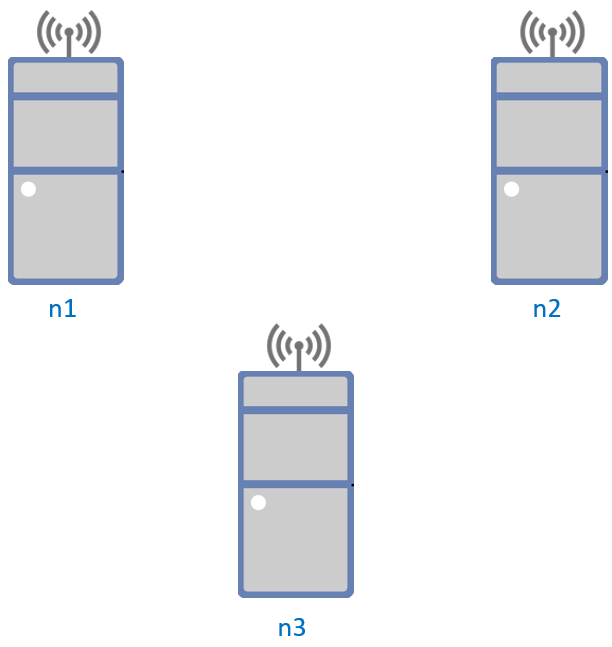
\includegraphics[width=0.5\linewidth]{graphics/ping-wireless-topology}	
		\caption{Wireless network topology in ping-example experiment.}
		\label{fig:lab7-ping-wireless}
	\end{figure}
	
	\begin{enumerate}
	\item Delete from the code everything related to the switch and wired links configuration. Note that pcap traces collection also has to be replaced, because we will not use the CsmaHelper anymore.
	
	\item Now we will add the Wi-Fi network configuration and install Wi-Fi NetDevices on each node. For that, we will use the following code:
	\begin{lstlisting}
	WifiHelper wifi;
	wifi.SetStandard (WIFI_STANDARD_80211a);
	SpectrumWifiPhyHelper wifiPhy;
	Ptr<MultiModelSpectrumChannel> channel = CreateObject<MultiModelSpectrumChannel>();
	wifiPhy.SetChannel (channel);
	WifiMacHelper wifiMac;
	wifiMac.SetType ("ns3::AdhocWifiMac", "QosSupported", BooleanValue (false));
	wifi.SetRemoteStationManager ("ns3::ConstantRateWifiManager",
	                              "DataMode",StringValue ("OfdmRate6Mbps"));
	NetDeviceContainer endNodeDevices = wifi.Install (wifiPhy, wifiMac, endNodes);
	\end{lstlisting}
	
	Here we configure separately Physical (PHY) and \ac{mac} layers of Wi-fi and pass them as arguments to the Install function of WiFiHelper. We explicitly set the constant rate mode, because by default Wi-Fi adapts its transmission rate depeding on nodes' channel conditions. We disable this feature and fix the transmission rate to 6 Mbps, which coresponds to the lowest Wi-Fi data rate. To make this code work, we have to include two libraries: \nolinkurl{ns3/wifi-module.h} and \nolinkurl{ns3/multi-model-spectrum-channel.h}.
	
	To enable pcap traces collection, instead of the prior line of code we add:
	\begin{lstlisting}
	wifiPhy.EnablePcapAll("ping-example")
	\end{lstlisting}
	
	\item Run the following command:
	\begin{cmdblock}[gobble=2]
		% git diff
	\end{cmdblock}
	You will see highlighted the differences you made in the file. Save the output of the command to a text file.
	
	\item Run the modified experiment. Make sure that the ArpCache::PopulateArpCache function call is added into the experiment source file. Save the program output and the generated pcap files.
	
	\question{Look inside the content of each pcap file. Which packets do you see inside them? Do all the pcap files contain the same packets? Why?}{0}
	
	\question{Look inside the content of the pcap file that corresponds to a source node that executes the ping command. How many packets are sent for each \ac{icmp} ping request?}{0}
	
	\question{Compare the results for the wireless and wired topologies. Use the pcap traces and saved text files. Please also indicate the name of the file that contains the output of the diff command.}{0}
	\end{enumerate}
\end{exercise}